\subsection{Object identification}
\label{sec:language-games:identification}

\subsubsection*{Setup}

The object identification game is set up as a discrimination game.
In a discrimination game, the agents are presented with two or more images, one of these being the target image.
The sender needs to communicate this target image to the receiver by discriminating it from the other distractor images.
The receiver then needs to decide based on the message, which of the images is the target image.

The discrimination games in this research have a very similar setup as described in \citep{Lazaridou2017}.
The agents in this research resemble their \emph{agnostic sender} as well as their \emph{receiver}.
One central difference is the production of the message.
The main goal of their language games was the identification of the concept that the shown image was related to.
Therefore, the sender communicated only single-symbol messages to the receiver which should describe the concept of the target image.
Opposed to that, in this research, the agents are tasked to discriminate objects from each other based on their attributes.
% SD: On the contrary,...
% DK: (done)
It is therefore assumed that the sender will communicate these discriminative attributes.
For that reason, the sender is allowed to generate sequences as a message where for instance each symbol in the sequence might correspond to one attribute.

The data is prepared in the same way as for the single model object identification task in section \ref{sec:object-identification}.
Bounding boxes of all objects in the scene are extracted and preprocessed to be used for the feature extractors.
For datasets with a variable number of objects, the list bounding of bounding boxes is padded with a matrix of zeros to the maximum possible number of objects present in a scene across the
dataset.
Opposed to the experiments with one neural model, no additional information about the target object's attributes is provided.
Instead, the sender agent is presented with the target object always as the first object, while the distractors are shuffled.
The receiver is presented with completely shuffled bounding boxes.

Accordingly, also the models from the single model tasks serve as basis for the object identification task.
The sender uses the architecture of the model described in section \ref{sec:referring_expression_generation} apart from the final LSTM.
Instead, it will use the LSTM with a hidden size $h_s$ included in the \emph{EGG} framework to produce a message.
Based on the results from the single model object identifiers, the image embedding size $e_s$ is fixed to 100.

The receiver instead uses the architecture of the single model object identifier, described in section \ref{sec:object-identification}.
Similarly to the sender, the LSTM of the \emph{EGG} framework with the hidden size $h_e$ is used to encode the sender's message instead of the one-hot encoded attributes in the single model.
The hidden state of the LSTM is projected to the embedding size $e_r=500$ with a linear layer, based on the results in the previous experiments.
As before the dot product between the embedded message and the encoded image is calculated to let the model point towards the bounding box that is described best by the message.
Figure \ref{fig:discriminator_architecture} shows, how the sender and the receiver of the discriminator are built up.

\begin{figure}[ht]
    \centering
    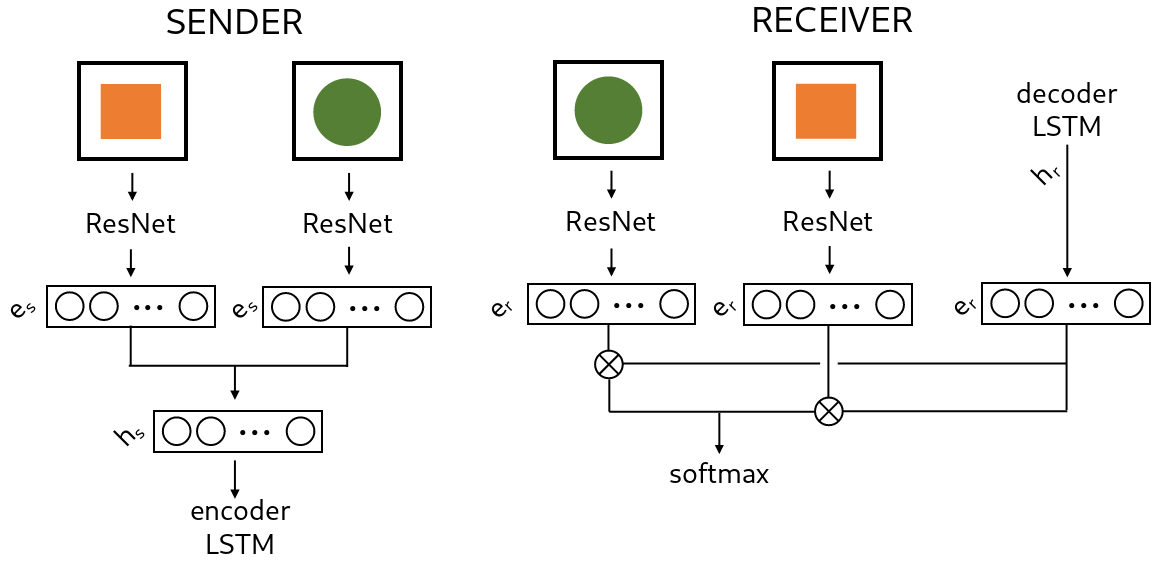
\includegraphics[width=.8\linewidth]{figures/arch_discriminator.png}
    \caption{Sender and receiver architectures in the discrimination game}
    \label{fig:discriminator_architecture}
\end{figure}

The experiments are conducted with a learning rate of $2\times10^{-4}$, the loss is calculated using cross entropy.
The following values for the variables are compared:
\begin{itemize}
    \item $h_s$: 100, 500, 1000
    \item $h_r$: 10, 30, 50, 100, 500, 1000
    \item $|V|$: 2, 10, 16, 50, 100
    \item $n$: 1, 2, 3, 4, 6
\end{itemize}

The language game is run on the 'Dale-2', 'Dale-5' and 'CLEVR color' datasets.
A random guess corresponds to 50\% in the \emph{Dale-2} dataset, 20\% in the \emph{Dale-5} dataset and 13\% in the \emph{CLEVR color} dataset.

\subsubsection*{Results}
When looking at the results of the experiments, it can be seen that the agents are successfully discriminating the objects across all datasets.
Table TODO gives an overview over the accuracy scores of selected configurations.
For each dataset there are many configurations that outperform the baseline models by a high margin.
However, there are still clear differences between the accuracy scores of each dataset.

When the agents are tasked to discriminate between the two objects of the \emph{Dale-2} dataset, it succeeds in almost all configurations with an accuracy of over 94\%.
In many configurations the accuracy lies above 99\%, while only 5 configurations have an accuracy of only 61\% to 64\%.
An indicator for



Table \ref{tab:results_discriminator} shows the accuracy of the models calculated on the success of communication if the receiver can identify the target object.

The hidden sizes $h_s$ and $h_r$ as well as the embedding sizes $e_s$ and $e_r$ are chosen in alignment with the vocabulary size.
The hidden sizes are always smaller or equal to the vocabulary size since the information about each word needs to be compressed in a smaller dimension to learn meaning.
Hereby, hidden sizes of 10 and 100 are tested.
On the other hand, three different embedding sizes are tested: 10, 50 and 100.
The reason for this is to experiment, what is the optimal middle ground between compressing features of an image encoded in high dimension vectors and upscaling encoded messages in low dimension vectors.
% SD: This discussion of dimensions could already be introduced when you discuss simple modles earlier as the same dimensions are used. This is a more an evaluation of represnetations rather than interaction and hence it would fit there.
% DK: TODO

\begin{table}[ht]
    \centering
    \begin{tabular}{ccccc|cc|cc|cc}
        \toprule
              &         &         &         &         & \multicolumn{2}{c}{\textbf{Dale-2}} & \multicolumn{2}{c}{\textbf{Dale-5}} & \multicolumn{2}{c}{\textbf{CLEVR color}}                                                         \\\cmidrule(lr){6-7}\cmidrule(lr){8-9}\cmidrule(lr){10-11}
        $|V|$ & $h_{s}$ & $h_{r}$ & $e_{s}$ & $e_{r}$ & \textbf{Accuracy}                   & \textbf{length}                     & \textbf{Accuracy}                        & \textbf{length} & \textbf{Accuracy} & \textbf{length} \\\midrule
        {10}  & {10}    & {10}    & {10}    & {10}    & {96,4\%}                            & {0,99}                              & {24,7\%}                                 & {0}             & {17,3\%}          & {1}             \\
        {10}  & {50}    & {50}    & {50}    & {50}    & {50\%}                              & {1}                                 & {21,4\%}                                 & {1}             & {17,8\%}          & {0}             \\
        {13}  & {10}    & {10}    & {10}    & {10}    & {96,16\%}                           & {1}                                 & {24,8\%}                                 & {1}             & {17,1\%}          & {1}             \\
        {13}  & {10}    & {10}    & {50}    & {50}    & {49,6\%}                            & {1}                                 & {21,9\%}                                 & {1}             & {17,9\%}          & {0}             \\
        {20}  & {10}    & {10}    & {50}    & {50}    & {50,9\%}                            & {0}                                 & {23\%}                                   & {1}             & {15,9\%}          & {1}             \\
        {100} & {10}    & {10}    & {10}    & {10}    & {97,3\%}                            & {1}                                 & {24\%}                                   & {1}             & {18,1\%}          & {1}             \\
        {100} & {10}    & {10}    & {50}    & {50}    & {49,9\%}                            & {1}                                 & {24,4\%}                                 & {1}             & {15,8\%}          & {1}             \\
        {100} & {100}   & {100}   & {100}   & {100}   & {49\%}                              & {0}                                 & {25,3\%}                                 & {1}             & {15,6\%}          & {0}             \\
        \bottomrule
    \end{tabular}
    \caption{Results of the discriminators: $|V|$ are different vocabulary sizes, $h$ hidden sizes and $e$ embedding sizes.}
    % SD: A note about the datasets chosen. Why do we choose these? Initially, we describe more than 3 datasets.
    % DK: because the 'CLEVR Single' contains only one object. So there is nothing to discriminate (done)
    \label{tab:results_discriminator}
\end{table}
% SD: As we discussed at Semdial, it would be good to have a learning curves here that would show how fast or slow the languages converge. As David pointed out it may be that convergence is unstable and changes happen in between.
% DK: TODO

For the \emph{Dale-2}, a clear correlation between the hidden sizes, embedding sizes and the size of the vocabulary can be identified.
A hidden/embedding size as high as the vocabulary size is beneficial for identifying the correct object.
The receiver identifies almost every sample correctly when all sizes are 10.
When the hidden and embedding sizes are increased, the guesses by the receiver are random with 50\% accuracy.
Interestingly, a vocabulary size of 10 is enough to communicate a meaningful message when the model is trained on the \emph{Dale-2} dataset.
% SD: How do we know? What would happen if the hidden layers are smaller than the vocabulary size? We would also need to test several smaller dimensions.
% DK: because the task is solved succesfully, TODO

The results change, when using the \emph{Dale-5} dataset with four distractors.
With four distractors and with low hidden, embedding and vocabulary sizes, the agents barely pass the random baseline with 23\%.
Only increasing the vocabulary size to 100 raises the accuracy by almost 20\% points to 43\%.
This is still considerably lower than the 95\% of the \emph{Dale-2} dataset.
The same applies to the 'CLEVR color' dataset, where all models achieve a very low accuracy of around 15 to 17\%, corresponding to random guesses.
% SD: Could we say that calculation on Dale-5 is successful?
% DK: TODO

Two conclusions can be drawn.
First, the hidden as well as the embedding sizes need to be close to the vocabulary size.
% SD: Not sure, since we never tested smaller layer sizes. If the embedding layers are the same as the vocabulary size then at least a language encoding LSTM is not motivated to geenralise at all as it can keep representations for individual words without abstracting them. Leanring word embeddings involves reducing dimensions.
% DK: TODO
This even applies for very low vocabulary sizes, which means that the image encodings need to be compressed to the same low dimensions.
The reason for this is very likely that neural models have difficulties to upscale from lower dimensions (e.g. from low $h_r$ to high $e_r$) as opposed to learn how to extract the important information from a vector with many dimensions.
% SD: Hypothesis space to find the target function is just too big and they can never approximate that function.
% DK: TODO

The second conclusion that can be drawn looks at the differences between the two datasets.
Unsurprisingly, the agents have a much higher difficulty to discriminate a target object from four instead of one distractor.
Since we discriminate objects based on properties that are also distinguished in human cognition (8 colors, 2 sizes, 3 shapes), we expect that the vocabulary onto which the agents converge reflects these categories and is therefore close to human vocabulary.
There are $8*2*3=48$ possible combinations of attributes.
% SD: Calculation behind this figure?
% DK: (done)
Still, for Dale-2, a vocabulary size of only 10 is enough for an almost perfect accuracy with two objects.
This hints to the fact that the agents don't describe the complete target object, but only rely on discriminative attributes between the objects.
The need for a more detailed description of discriminative attributes is higher when more distractors are involved.
Therefore, the models need to learn more combinations of symbols in order to attest to this higher level of detail and especially how to relate them to features in the images.
% SD: We would need to show that the messages in Dale-2 are shorter than in Dale-5 to claim this.
% DK: TODO

\cmtDK[inline]{similarity to bounding box classifier}
